% VUT FIT MITAI
% MSZ 2021/2022
% Author: Vladimir Dusek
% Login: xdusek27

%%%%%%%%%%%%%%%%%%%%%%%%%%%%%%%%%%%%%%%%%%%%%%%%%%%%%%%%%%%%%%%%%%%%%%%%%%%%%%%%

% Path to figures
\graphicspath{{pds/pds_prerekvizity/figures}}

%%%%%%%%%%%%%%%%%%%%%%%%%%%%%%%%%%%%%%%%%%%%%%%%%%%%%%%%%%%%%%%%%%%%%%%%%%%%%%%%

\chapter{PDS~--~Prerekvizity k ostatním otázkám.}

%%%%%%%%%%%%%%%%%%%%%%%%%%%%%%%%%%%%%%%%%%%%%%%%%%%%%%%%%%%%%%%%%%%%%%%%%%%%%%%%

% \section{Zdroje}

% \begin{compactitem}
%     \item \todo{todo}
% \end{compactitem}

%%%%%%%%%%%%%%%%%%%%%%%%%%%%%%%%%%%%%%%%%%%%%%%%%%%%%%%%%%%%%%%%%%%%%%%%%%%%%%%%

\paragraph*{ISO/OSI model} Referenční model ISO/OSI se používá jako názorný příklad řešení komunikace v počítačových sítích pomocí vrstevnatého modelu, kde jsou jednotlivé vrstvy nezávislé a snadno nahraditelné. \begin{compactitem}

    \item \textbf{Aplikační vrstva} (L7, \textit{application layer}) \begin{compactitem}
        \item Zajišťuje zpracování dat na nejvyšší úrovni (reprezentace dat, kódování, řízení dialogu, \dots).
        \item Tvořena procesy a aplikacemi, které komunikují po síti.
        \item Bývá slučována s prezentační vrstvou (L6, prezentace dat a šifrování) a relační vrstvou (L5, koordinace a komunikace).
        \item Příklad protokolů: \begin{compactitem}
            \item Uživatelské~--~vykonávají služby přímo uživateli (Telnet, SSH, FTP, SMTP, HTTP, \dots)
            \item Systémové~--~zajišťují síťové funkce (DNS, DHCP, SNMP, BOOTP, \dots)
        \end{compactitem}
    \end{compactitem}

    \item \textbf{Transportní vrstva} (L4, \textit{transport layer}) \begin{compactitem}
        \item Rozděluje aplikační data (segmentace) na menší jednotky a zapouzdřuje je do segmentů (TCP) / datagramů (UDP).
        \item Vytváří logické spojení mezi procesy (přenáší data konkrétní aplikace ze zdrojového zařízení do aplikace na cílovém zařízení).
        \item Adresace: porty.
        \item Příklad protokolů: TCP, UDP, DCCP, SCTP, MP-TCP, QUIC
    \end{compactitem}

    \item \textbf{Síťová vrstva} (L3, \textit{network layer}) \begin{compactitem}
        \item Zapouzdřuje segmenty/datagramy do paketů.
        \item Řeší směrování.
        \item Adresace: IP adresa (logická adresa).
        \item Příklad protokolů: IPv4, IPv6, ARP, RARP, ICMP, IGMP
    \end{compactitem}

    \item \textbf{Linková vrstva} (L2, \textit{data link layer}, vrstva síťového rozhraní, \textit{network interface layer}) \begin{compactitem}
        \item Zapouzdřuje pakety do rámců.
        \item Zajišťuje \textit{hop-by-hop} doručení.
        \item Adresace: MAC adresa (fyzická adresace).
        \item Příklad protokolů: Ethernet, Token Ring, FDDI, X.25, Frame Relay
    \end{compactitem}

    \item \textbf{Fyzická vrstva} (L1, \textit{physical layer}) \begin{compactitem}
        \item Zajišťuje přenos bitů přes fyzické médium.
    \end{compactitem}
\end{compactitem}

\paragraph*{Adresace} \begin{compactitem}
    \item Port (transportní vrstva, L4) \begin{compactitem}
        \item Identifikuje aplikaci v rámci zařízení.
        \item Jak se mění při směrování paketu internetem: zůstává stejný s výjimkou zdrojového portu při překladu NAT.
        \item Velikost: 16 bit
        \item Prostor: plochý
    \end{compactitem}
    \item IPv4, IPv6 (síťová vrstva, L3) \begin{compactitem}
        \item Identifikuje uzel v rámci sítě (tzv. logická adresace).
        \item Jak se mění při směrování paketu internetem: zůstává stejná s výjimkou zdrojové IP adresy při překladu NAT.
        \item Velikost: 32 bit, 128 bit
        \item Prostor: pseudohierarchie (A, B, C, D, E), pseudohierarchie (prefix + interface ID)
    \end{compactitem}
    \item MAC (linková vrstva, L2) \begin{compactitem}
        \item Identifikuje síťové rozhraní (síťovou kartu).
        \item Jak se mění při směrování paketu internetem: mění se \textit{hop-by-hop}.
        \item Velikost: 32 bit, 128 bit
        \item Prostor: pseudohierarchie (A, B, C, D, E), pseudohierarchie (prefix + interface ID)
    \end{compactitem}
\end{compactitem}

\paragraph*{data, segment, datagram, paket, rámec, bit} \begin{compactitem}
    \item Data~--~aplikační vrstva (L7)
    \item Segment~--~transportní vrstva (L4), TCP
    \item Datagram~--~transportní vrstva (L4), UDP
    \item Paket~--~síťová vrstva (L3)
    \item Rámec~--~linková vrstva (L2)
    \item Bit~--~fyzická vrstva (L1)
\end{compactitem}

% src: https://linuxhint.com/network-osi-layers-explained
\begin{figure}[H]
    \centering
    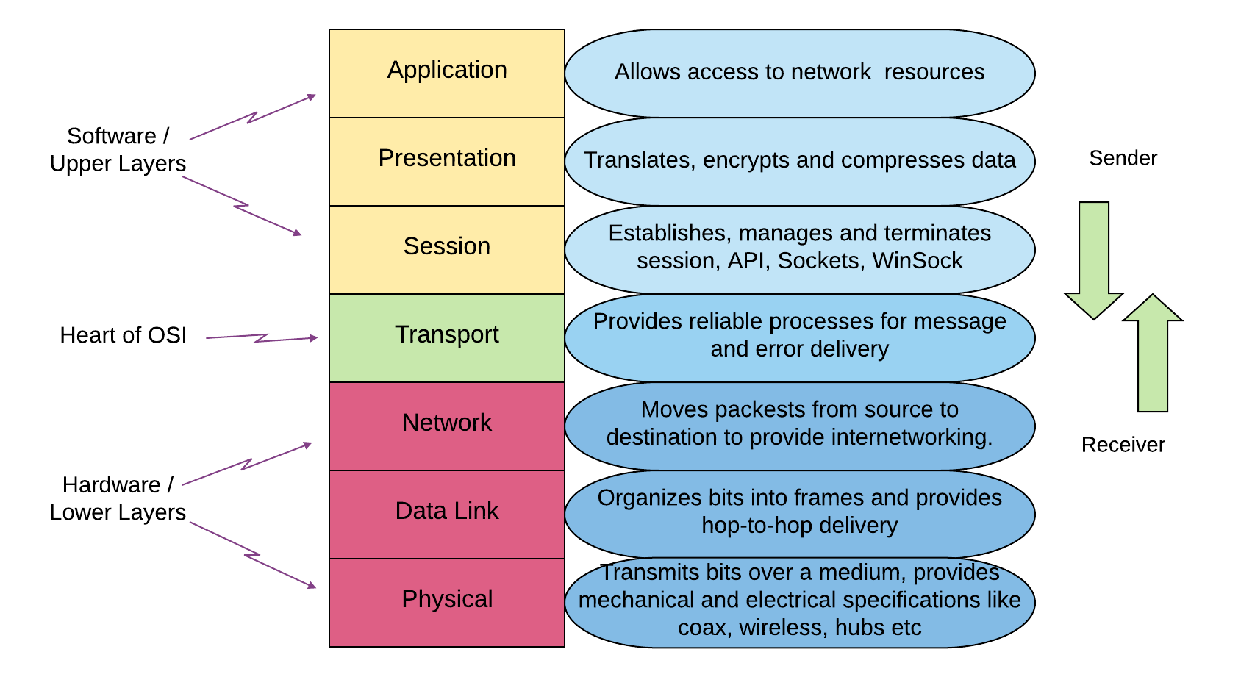
\includegraphics[width=1\linewidth]{osi_model_linuxhint.pdf}
    \caption{Příklad OSI modelu z Linuxhint.}
\end{figure}

% src: https://cs.wikipedia.org/wiki/Soubor:OSI_Model_v1.svg
\begin{figure}[H]
    \centering
    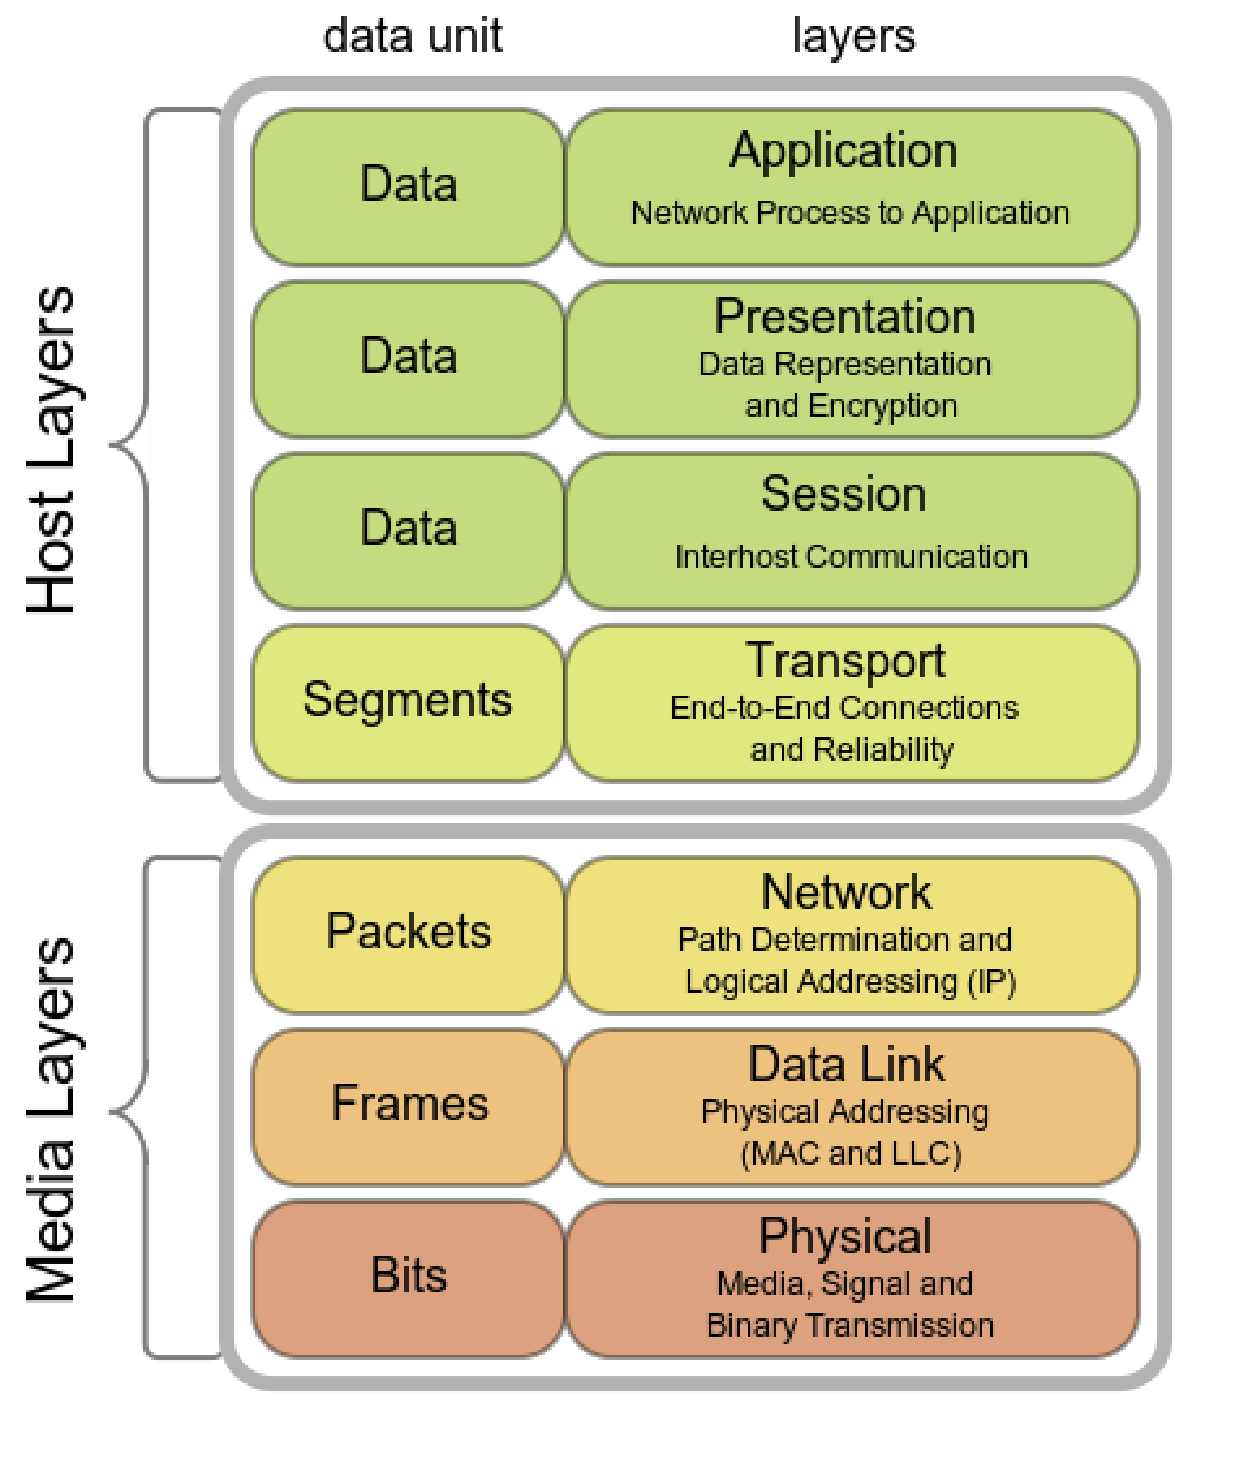
\includegraphics[width=0.65\linewidth]{osi_model_wiki.pdf}
    \caption{Příklad OSI modelu z Wiki.}
\end{figure}

\paragraph*{ACL} ACL (\textit{Access Control List}) je volitelná vrstva zabezpečení, která funguje jako brána firewall pro řízení provozu do jedné nebo více podsítí a z nich.

\paragraph*{NAT} NAT (\textit{Network Address Translation}) je metoda mapování IP adresního prostoru do jiného prostoru (typicky privátní adresy na veřejné adresy). Děje se tak úpravou hlaviček IP paketů během jejich přenosu přes směrovače (úprava zdrojové IP adresy a čísla portu). Směrovač si ukládá čtveřice $(\text{WAN\_IP}:\text{WAN\_port}, \text{LAN\_IP}:\text{LAN\_port})$ aby mohl prováděť i překlad zpět.

\paragraph*{ARP} ARP (\textit{Address Resolution Protocol}) a RARP (\textit{Reverse ARP}) je protokol, který komunikuje na síťové vrstvě (L3) a zajišťuje \uv{překlad} IP adres na MAC adresy a obráceně. Pouze pro IPv4, pro IPv6 je pro stejný účel využíván protokol ICMPv6 a zpráva \textit{Neighbor Discovery}. Příklad využití: směrovač potřebuje získat MAC adresu next hopu (zná jeho IP adresu).

\paragraph*{ICMP} ICMP (\textit{Internet Control Message Protocol}) je protokol, který komunikuje na síťové vrstvě (L3) a slouží pro řízení toku a detekce nedosažitelných uzlů.

\paragraph*{MAC adresa} MAC adresa je fyzická adresa zařízení, resp. síťové karty (identifikátor na L2). Na každý síťový port v přepínači/směrovači je jedna síťová karta (a teda i MAC adresa).

% Todo: lepe, toto neni moc pravda
\paragraph*{IP adresa} IP adresa je logická adresa zařízení (identifikátor na L3). Pokud má zařízení více síťových karet, má typicky stále pouze jednu IP adresu. Přepínač nemá IP adresu vůbec, pracuje pouze na L2 vrstvě. Směrovač je výjimka a má 2 IP adresy, jednu pro komunikaci v lokální síti (LAN) a druhou pro internet (WAN).

\paragraph*{Síťový tok} Síťový tok je posloupnost paketů (jednosměrná) identifikována čtveřicí (zdrojová IP, zdrojový port, cílová IP, cílový port).

\begin{figure}[H]
    \centering
    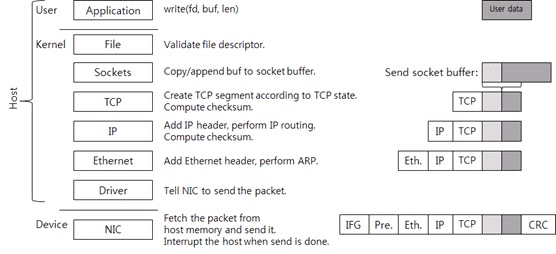
\includegraphics[width=1\linewidth]{operation_process_by_each_layer.png}
    \caption{Operace na jednotlivých vrstvách ISO modelu.}
\end{figure}
